
\noindent 
\begin{homework}
	Verify that $R_{ij} = R_{ji}^{-1} \equiv R_{ji}^T$. Furthermore, verify that the determinant of the rotation matrix is $\pm1$ \ie $det R = \pm1$.
\end{homework}

\begin{solution}
	We have 
%
\begin{align}
R_{ij} &= 	\begin{bmatrix}
	\bm{x}_i \cdot \bm{x}_j & \bm{y}_i \cdot \bm{x}_j & \bm{z}_i \cdot \bm{x}_j \\
	%
	\bm{x}_i \cdot \bm{y}_j & \bm{y}_i \cdot \bm{y}_j & \bm{z}_i \cdot \bm{y}_j \\
	%
	\bm{x}_i \cdot \bm{z}_j & \bm{y}_i \cdot \bm{z}_j & \bm{z}_i \cdot \bm{z}_j 
	\end{bmatrix},
	\label{eq:rot}
	\end{align} 
	%
	\begin{align}
	R_{ji} &= 	\begin{bmatrix}
	\bm{x}_j \cdot \bm{x}_i & \bm{y}_j \cdot \bm{x}_i & \bm{z}_j \cdot \bm{x}_i \\
	%
	\bm{x}_j \cdot \bm{y}_i & \bm{y}_j \cdot \bm{y}_i & \bm{z}_j \cdot \bm{y}_i \\
	%
	\bm{x}_j \cdot \bm{z}_i & \bm{y}_j \cdot \bm{z}_i & \bm{z}_j \cdot \bm{z}_i 
	\end{bmatrix},
	\label{eq:rot_rev}
	\end{align}	
	%
	and that
	%
\begin{align}
	R_{ji}^T & = 
	\begin{bmatrix}
	\bm{x}_j \cdot \bm{x}_i & \bm{x}_j \cdot \bm{y}_i  & \bm{x}_j \cdot \bm{z}_i \\
	%
	\bm{y}_j \cdot \bm{x}_i & \bm{y}_j \cdot \bm{y}_i & \bm{y}_j \cdot \bm{z}_i \\
	%
	\bm{z}_j \cdot \bm{x}_i & \bm{z}_j \cdot \bm{y}_i  & \bm{z}_j \cdot \bm{z}_i 
	\end{bmatrix}.
	\end{align}
	%
	Inspecting the rows of $R_{ij}$ and $R_{ij}^T$, the dot products between the respective vector elements are simply the cosine of the angles between them \ie $p_j \cdot p_i = cos \theta$, where $\theta$ is the angle between the vectors $p_j$ and $p_i$. Evaluating, it follows that $R_{ij}^T = R_{ij}$. Similarly, we know that a matrix $X$ is invertible if there exists a matrix $B$ such that
	%
	\begin{align}
		AB = BA = \identity_n
	\end{align}
	%
	where $I_n$ is an $n \times n$ matrix. In this case, we have that 
	%
	\begin{align}
	R_{ji} R_{ji}^T = R_{ji}^T R_{ji} = \identity_3.
	\end{align}
	%
	It follows that, 
	%
	\begin{align}
	R_{ji} = \dfrac{1}{R_{ji}^T}
	\end{align}
	%
	or 
	\begin{align}
	R_{ji}^T = R_{ji}^{-1}. 
	\end{align}
	%
	From \eqref{eq:rot} and \eqref{eq:rot_rev}, it follows that see that
	%
	\begin{align}
	R_{ji}^T = R_{ji}^{-1} = R_{ij}. 
	\end{align}
\end{solution}


\begin{homework}
	Compose the rotation matrix in three dimensions where all axes of the inertial frame are rotated by an angle $\beta$ around each of the $x_0$, $y_0$ and $z_0$ axes respectively using the foregoing logic. In addition, for each transformation, verify that (1) $R_{e, 0} = I$\footnote{In your notes, this was written as $R_{e, \beta}$. You will not be penalized if you could not arrive at the right solution because of this mistake.} where $e$ is the axes about which we are rotating and $\beta$ is the angle of rotation, (2) the composition of rotations about the angles $\beta$ and $\alpha$ in a successive manner implies that $R_{z, \beta}, R_{z, \alpha} = R_{z, \beta + \alpha}$, and (3) ${(R_{z, \beta})}^{-1} = R_{z, -\beta}$. Bonus points will be awarded for cool 3D visualizations.
\end{homework} 

\begin{solution}
	In three dimensions, a rotation angle of $\beta$ around the principal axes of the moving frame  $x_0, y_0, z_0$, gives the rotation matrix
	%
	\begin{align}
	\begin{bmatrix}
	\bm{x}_1 \cdot \bm{x}_0 & \bm{y}_1 \cdot \bm{x}_0   &   \bm{z}_1 \cdot \bm{x}_0  \\
	%
	\bm{x}_1 \cdot \bm{y}_0    & \bm{y}_1 \cdot \bm{y}_0   &  \bm{z}_1  \cdot  \bm{y}_0 \\
	%
	 \bm{x}_1\cdot  \bm{z}_0   &   \bm{y}_1 \cdot \bm{z}_0  &  \bm{z}_1 \cdot \bm{z}_0
	\end{bmatrix} 
	%
	\end{align}
	%	
	A rotation about $x$ by $\beta$ gives,
	%
	\begin{align}
	R_{x_0, \beta} = \begin{bmatrix}
	1 & 0   &  0  \\
	%
	0   & \cos \beta   &  -\sin \beta  \\
	%
	0  &  \sin \beta  &  \cos \beta 
	\end{bmatrix},
	\label{eq:rbx}
	\end{align}
	%
	a rotation about $y_0$ by $\beta$ gives,
	%
	\begin{align}
	R_{y_0, \beta} = \begin{bmatrix}
	\cos \beta & 0   &  \sin \beta   \\
	%
	0   &  1   &  0 \\
	%
	-\sin \beta  &  0  &  \cos \beta 
	\end{bmatrix}
	\label{eq:rby}
	\end{align}
	%
	and a rotation about $z_0$ by $\beta$ gives,
	%
	\begin{align}
	R_{z_0, \beta} = \begin{bmatrix}
	\cos \beta & -\sin \beta    &  0  \\
	%
	\sin \beta    &  \cos \beta   &  0 \\
	%
	0 &  0  &  1 
	\end{bmatrix}.
	\label{eq:rbz}
	\end{align}
	%
	Substituting $0$ for $\beta$ in \eqref{eq:rbx}, \eqref{eq:rby}, and \eqref{eq:rbz}, we have
	%
	\begin{align}
		R_{x_0, \beta} = R_{\beta, y_0} = R_{\beta, z_0} = \begin{bmatrix}
		1 & 0   &  0  \\
		%
		0    &  1   &  0 \\
		%
		0 &  0  &  1 
		\end{bmatrix}.
	\end{align}
	
	The composition of rotations about the angles $\beta$ and $\alpha$ in a successive manner implies that $R_{z, \beta}  R_{z, \alpha} = R_{z, \beta + \alpha}$
	
	\noindent \textbf{Proof}: 
	\begin{align}
		R_{\beta, z_0} R_{\alpha, z_0}  &= \begin{bmatrix}
		\cos \beta & -\sin \beta    &  0  \\
		%
		\sin \beta    &  \cos \beta   &  0 \\
		%
		0 &  0  &  1 
		\end{bmatrix} \, \begin{bmatrix}
		\cos \alpha & -\sin \alpha    &  0  \\
		%
		\sin \alpha    &  \cos \alpha   &  0 \\
		%
		0 &  0  &  1 
		\end{bmatrix} \\ 
		%
	R_{\beta, z_0} R_{\alpha, z_0}	&= \begin{bmatrix}
		c_\alpha c_\beta -s_\alpha s_\beta & c_\alpha s_\beta -c_\beta s_\alpha    &  0  \\
		%
		c_\alpha s_\beta + s_\alpha c_\beta    &  c_\alpha c_\beta - s_\alpha s_\beta  &  0 \\
		0 & 0 & 1
		\end{bmatrix} .
	\end{align}
	%
	or 
	\begin{align}
	R_{\beta, z_0} R_{\alpha, z_0}	&= \begin{bmatrix}
		\cos(\alpha + \beta) & -\sin(\alpha + \beta)    &  0  \\
		%
		\sin(\alpha + \beta)     &  \cos(\alpha + \beta)  &  0 \\
		0 & 0 & 1
	\end{bmatrix} .
	\label{eq:rot_a_then_b}
\end{align}

Now, we find that 
%
\begin{align}
	R_{z, \beta + \alpha} = \begin{bmatrix}
	\cos(\alpha + \beta) & -\sin(\alpha + \beta)    &  0  \\
	%
	\sin(\alpha + \beta)     &  \cos(\alpha + \beta)  &  0 \\
	0 & 0 & 1
	\end{bmatrix}.
	\label{eq:rot_a_plus_b}
\end{align}
%
Since \eqref{eq:rot_a_then_b} = \eqref{eq:rot_a_plus_b}, the supposition is confirmed.

\noindent \textbf{Prove that ${(R_{z, \beta})}^{-1} = R_{z, -\beta}$}:
%
We have from \eqref{eq:rbz} that
%
\begin{align}
R_{z, -\beta} = \begin{bmatrix}
\cos(-\beta )& -\sin (-\beta)    &  0  \\
%
\sin (-\beta)    &  \cos (-\beta)   &  0 \\
%
0 &  0  &  1 
\end{bmatrix} = \begin{bmatrix}
\cos(\beta )& \sin (\beta)    &  0  \\
%
-\sin (\beta)    &  \cos (\beta)   &  0 \\
%
0 &  0  &  1 
\end{bmatrix}.
\end{align}

Now, $(R_{z, \beta})^{-1}$ = $(R_{z, \beta})^T$ so that 
%
\begin{align}
	R_{z, \beta}^T = \begin{bmatrix}
	\cos \beta & \sin \beta    &  0  \\
	%
	-\sin \beta    &  \cos \beta   &  0 \\
	%
	0 &  0  &  1 
	\end{bmatrix}.
\end{align}
%
The equivalence of the two preceding equations prove our case. (QED)
\end{solution}

\begin{figure}[tb!]
	\centering
	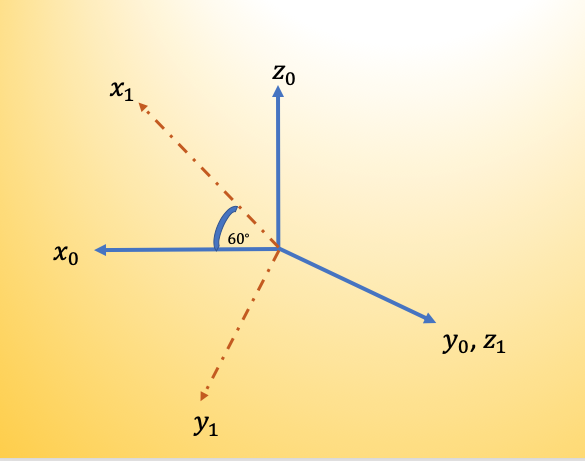
\includegraphics[width=.8\columnwidth]{../lec_notes/figures/two_frames.png}
	\caption{Relative orientation between two frames.}
	\label{fig:two_frames}
\end{figure}


\noindent 
\begin{homework}
	For the two frames shown in \autoref{fig:two_frames}, determine the rotation matrix between them. In addition, explain the difference between rotating about a \textit{current frame} and rotating about a \textit{fixed frame}\footnote{See sections 2.4.1 and 2.4.2 of Spong's book.}. In particular, when is it necessary to carry out a \textit{pre-multiplication} and when is it necessary to carry out a \textit{post-multiplication} when transforming points or vectors about coordinate frames?
\end{homework}

\begin{solution}
	From the given figure, observe that the $x_0$ axis was rotated counterclockwise by $60^\circ$ from the horizontal. To find the rotation matrix between the two frames, we can project the unit vectors $x_1, y_1, z_1$ onto $x_0, y_0, z_0$ to generate the coordinates of $x_1, y_1, z_1$ in the $x_0, y_0, z_0$ frame. We therefore have
	%
	\begin{align}
		x_1 = \begin{bmatrix}
		\frac{1}{2} 
		\\
		0
		\\
		\frac{\sqrt{3}}{2}
		\end{bmatrix}, \quad
		%
		y_1 = \begin{bmatrix}
		\frac{\sqrt{3}}{2}
		\\
		0
		\\
		-\frac{\sqrt{3}}{2}
		\end{bmatrix},  \quad
		%
		z_1 = \begin{bmatrix}
		0
		\\
		1
		\\
		0
		\end{bmatrix}
	\end{align}
\end{solution}


\noindent 
\begin{homework}
	For the robot manipulator we are using in this class, suppose that you have the following point in the base frame of the robot, $q_o = [-2, 3, 1]$. Furthermore, suppose that the joint angles for all six joints are respectively $\{-90, 60, 30, 45, 90, 125 \}$, transform the point $q_0$ in the base frame to a coordinate frame on the sixth joint.
\end{homework}

\begin{solution}
Since we changed the robot we are using, this homework is rendered moot and you will not be graded for it.
\end{solution}

Consider the composition of rotations of \autoref{fig:compoz} where we first rotate by an angle $\theta$ about the $x$ axis and then rotate about an angle $\psi$ about the $z$ axis. The rotation matrix can be composed as 
%
\begin{figure}[tb!]
	\centering
	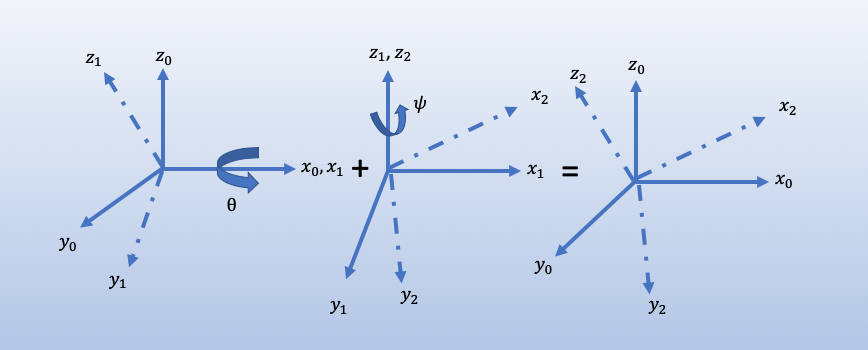
\includegraphics[width=\columnwidth]{../lec_notes/figures/compoz.png}
	\caption{Illustration of composition of rotations about a \textbf{current axis}.}
	\label{fig:compoz}
\end{figure}
%
\begin{align}
R &= R_{x, \theta} R_{z, \psi} 
%
&= \left(\begin{array}{ccc}
1 & 0 & 0 \\
0 & c_\theta & -s_\theta \\
0 & s_\theta & c_\theta
\end{array}\right) 
%
\cdot
%
\left(\begin{array}{ccc}
c_\psi & -s_\psi & 0 \\
s_\psi & c_\psi & 0 \\
0 & 0 & 1
\end{array}\right)
\end{align}
%
\begin{align}
R	&= \left(\begin{array}{ccc}
	c_\psi & -s_\psi & 0 \\
	c_\theta s_\psi & c_\theta c_\psi &  -s_\theta \\
	s_\theta s_\psi & s_\theta c_\psi & c_\theta 
	\end{array}\right)
\end{align}
Notice how the order of multiplication is carried out, owing to the axis about which we are making the transformation. 

\noindent 
\begin{homework}
	Carry out the transformation above in reverse order. What do you notice?
\end{homework} 

\begin{solution}
	Reversing the order of transformation reveals that
	\begin{align}
 R_{z, \psi} R_{x, \theta}=
	%
	\left(\begin{array}{ccc}
	c_\psi & -s_\psi & 0 \\
	s_\psi & c_\psi & 0 \\
	0 & 0 & 1
	\end{array}\right)
	%
	\cdot
	%
	 \left(\begin{array}{ccc}
	1 & 0 & 0 \\
	0 & c_\theta & -s_\theta \\
	0 & s_\theta & c_\theta
	\end{array}\right) 
	\end{align}
	%
	\begin{align}
		R &=  R_{z, \psi} R_{x, \theta} = \left(\begin{array}{ccc}
		c_\psi & -c_\theta s_\psi & s_\psi s_\theta \\
		s_\psi & c_\psi c_\theta  & - c_\psi s_\theta \\
		0 & s_\theta & c_\theta
		\end{array}\right)
	\end{align}
	\ie $R_{x, \theta} R_{z, \psi} = (R_{x, -\theta} R_{z, -\psi})^T $
\end{solution}
%
which goes to show that reversing the order of rotations is tantamount to reversing the order of angle rotations and then taking the transpose of the ensuing result. 